\newtheorem{conj}{Conjecture}[section]

\chapter{Graph Properties}
\label{ch:graph}

In the previous chapter we proved lower query bounds for Boolean
functions whose outputs show symmetry with respect to the Hamming
weight of the inputs.  We now consider lower bounds for graph
properties.  In Section \ref{sec:prelim} we cover the definitions of
deterministic decision trees, evasiveness and graph properties, and
formalize how we will represent graphs as bit strings so that we may
examine them in the oracle query model. We also present the
Aanderaa-Karp-Rosenberg conjecture, which motivates the study of
non-trivial monotone graph properties in particular.

We apply the result of Section \ref{sec:lqbsym} with limited success
to generic non-trivial monotone graph properties in Section
\ref{sec:lqbnmgp}.  We then apply Ambainis' Theorem \ref{th:amb} to 
attain new lower bounds of $\Omega(V)$ for computing connectivity and
bipartiteness in Sections \ref{sec:gc} and \ref{sec:bip}.  The lower
bounds attained for these problems leads us to question if there is a
quantum extension of the Aanderaa-Karp-Rosenberg conjecture in the
quantum bounded error setting, in Section \ref{sec:arkbad} we
establish that there is not.

\section{Preliminaries}
\label{sec:prelim}

\paragraph{Deterministic Decision Trees:}
\label{subs:ddt}

A decision tree of $N$ bits is a rooted binary tree.  Each internal
node of the tree contains an index $i \in \{1, \ldots, N\}$ and has
two children.  Each leaf contains either a $1$ or a $0$. To determine
the value of the deterministic decision tree on an input $x
\in \{0,1\}^{N}$ we traverse the tree starting at the root.  At each
internal node we examine the $x_{i}$, where $i$ is the index stored at
that node.  If $x_{i} = 1$ we follow the path through the left
subtree; if $x_{i} = 0$ we follow the path through the right subtree.
The value stored at the leaf that we eventually reach is the output of
the algorithm.  Any decision tree computes an $N$-bit Boolean
function.  There are many different deterministic decision trees that
compute any given function.

\label{subs:ddtc}

The decision tree complexity of a Boolean function is the minimum
depth of any decision tree that computes that function.  We denote the
decision tree complexity of a Boolean function $f$ by $D(f)$.  The
decision tree complexity of a function $f$ is just its classical
oracle query complexity.  Any decision tree of depth $D(f)$ determines
a minimal sequence of oracle queries that allow us to compute $f(x)$
for any input $x$.

\paragraph{Evasive Functions:}
\label{sec:ef}
Any $N$-bit Boolean function $f$ has a deterministic decision tree
complexity associated with it.  An $N$-bit Boolean function is
\emph{evasive} if and only if its deterministic decision tree
complexity is $N$.  Some evasive graph properties are connectivity,
bipartiteness, is the graph a tree, and does the graph have $k$ edges.

Evasive functions are then the hardest problems in the classical
oracle query model; for some input we are required to examine every
possible edge.  The nonconstant symmetric functions AND, OR, MAJORITY,
and PARITY of Section \ref{sec:AOMP} are evasive; indeed, all
nonconstant symmetric function are evasive (consider two consecutive
Hamming weights the function differs on, $a$ and $a+1$, the adversary
answers $1$ to the first $a$ queries, and $0$ to the rest).

\paragraph{Graph Properties:}
\label{sec:gp}
A graph property is a set of graphs closed under graph isomorphism.
If a graph property holds for some graph $G$, it must hold for all
graphs $G^{\prime}$ isomorphic to $G$.  For example: ``Is there an
edge from vertex 1 to vertex 2?'' is not a graph property, but ``Does
the graph have one edge?'' is.  Some graph properties are symmetric,
such as ``Is the graph complete?''  Others exhibit symmetry in a
different sense than that of Definition \ref{def:sym}, such as ``Does
the graph contain a vertex of degree 5?''

A non-trivial graph property is one that is false for some graph, and
true for some graph.  If adding an edge to a graph can not make a
property fail the graph property is called \emph{monotone}.  Examples
of well-known monotone graph properties are whether a graph is
connected, acyclic, non-bipartite, complete, non-planar, or
non-$k$-colorable.  Nonmonotone graph properties include whether the
graph is a tree and $k$-regularity.

\begin{conj}[Aanderaa-Karp-Rosenberg]
\label{cj:ark}
All non-trivial monotone graph properties are evasive in the classical
deterministic setting.
\end{conj}

Conjecture \ref{cj:ark} is known to be true for graphs whose number of
vertices is a prime power \cite{lovasz94evasive}.

The conjecture makes monotone graph properties an appealing target for
study in the quantum oracle model.  We attained asymptotically tight
lower bounds for evasive symmetric functions in Chapter
\ref{ch:oracle}.  In non-trivial monotone graph properties we have a
class of functions, conjectured to be evasive, that exhibit a kind of
symmetry due to their invariance under relabeling of vertices.  We
hope that Ambainis' Theorem can provide us with asymptotically tight
lower bounds for non-trivial monotone graph properties as they did for
nonconstant symmetric functions.

\paragraph{Representing Graphs as Bit Strings:}
\label{sec:gbs}

Before we begin we need a way to represent a graph as a bit string,
and graph properties as Boolean functions on that bit string if we
wish to apply Theorem \ref{th:amb} or any of its derivatives.  When
representing graphs as bit strings it is helpful to restrict the types
of graphs we will consider.

A simple graph has no multiple edges or loops.  The adjacency matrix
$A$ of a simple directed graph has $a_{ij} = 1$ if and only if there
is a directed edge from vertex $i$ to vertex $j$.  Since $a_{ii} = 0$
for all vertices $i$ of a simple graph, we need only $V(V-1)$ bits to
represent such graphs with $V$ vertices.  For undirected graphs, the
adjacency matrix is symmetric across the diagonal.  Thus we can
represent any undirected simple graph with a bit string of length
$V(V-1)/2$.  A simple undirected graph is depicted in Figure
\ref{fi:graph}, its above-diagonal adjacency matrix representation can
be seen in Table \ref{tbl:graph}.  Now that we can represent a graph
by its above diagonal adjacency matrix, graph properties are simply
Boolean functions on matrix representations.

\begin{figure}
\begin{center}
\includegraphics{figures/sample_graph.eps}
\caption{An Undirected Graph \label{fi:graph}}
\end{center}
\end{figure}


\begin{table}
\begin{center}
\(\begin{array}{cccccc}
	  & B & C & D & E & F \\ A & 1 & 1 & 0 & 0 & 0 \\ B & & 1 & 1
	  & 0 & 0 \\ C & & & 0 & 0 & 0 \\ D & & & & 1 & 1 \\ E & & & &
	  & 0
\end{array}\)
\caption{Above Diagonal Adjacency Matrix Representation of the Graph in Figure \protect\ref{fi:graph} \label{tbl:graph}}
\end{center}
\end{table}

\section{Non-trivial Monotone Graph Properties}
\label{sec:lqbnmgp}	

For a non-trivial monotone graph property $p$, there exists some $a <
b$ such that the property holds for all graphs with $b$ edges, but not
for any graph with $a$ edges.  We can therefore apply Theorem
\ref{th:ptsym}.  While this may yield a good lower bound, sometimes it
will give us a trivial $\Omega(1)$ lower bound.

\subsection{Graph Connectivity}
\label{sec:gc}

One of the most fundamental non-trivial monotone graph properties is
graph connectivity.  Graph connectivity is known to be evasive
\cite{felsner92complexity}, so $V(V-1)/2$ oracle queries are 
required to decide graph connectivity for a simple undirected graph in
the classical case.

Every graph with $V-2$ edges is unconnected, and every graph with
$(V-1)(V-2)/2$ edges is connected.  We can apply Theorem
\ref{th:ptsym} with $a = V-2$, $b = (V-1)(V-2)/2$, and $N =
V(V-1)/2$.  This gives us only the trivial lower bound
\[\Omega\left(\sqrt{\frac {\left(\frac{V(V-1)}{2} -
(V-2)\right)\left(\frac{V(V-1)}{2} - (V-2)\right) }
{\left(\frac{V(V-1)}{2} - (V-2) - (V-2)\right)^{2}}}
\right) = \Omega(1).\] 
However, through better choices of the sets $X$ and $Y$ and the
relation $P$ for Theorem \ref{th:amb} we will prove that $\Omega(V)$
oracle queries are required to compute graph connectivity in the
bounded error setting.

To prove a lower bound for graph connectivity we will need Lemmas
\ref{lm:1erc} and \ref{lm:1ernc}, which delineate classes of connected 
and unconnected graphs whose number of edges differ by one.

\begin{lemma}
\label{lm:1erc}
If the above diagonal adjacency matrix representation of a simple
undirected graph has exactly one 1 in each row then the graph it
represents is connected.
\end{lemma}

\begin{proof}
There is a path from every vertex to vertex $V$, and there are $V-1$
edges, therefore the graph is a tree.  Trees are connected.
\end{proof}

\begin{lemma}
\label{lm:1ernc}
If the above diagonal adjacency matrix representation of a simple
undirected graph has exactly one 1 in each row except one row which
has all 0's then the graph it represents is not connected.
\end{lemma}

\begin{proof}
No graph with $V-2$ edges is connected.
\end{proof}

\begin{theorem}
\label{th:gc}
$\Omega(V)$ oracle queries are required to decide whether a simple
undirected graph is connected in the bounded error setting.
\end{theorem}

\begin{proof}
We apply Theorem \ref{th:amb}, we consider only simple undirected
graphs with $V \ge 3$. 

Let $X$ be the graphs whose adjacency matrix has exactly one 1 in each
row.  By Lemma \ref{lm:1erc} all such graphs are connected. Let $Y$ be
the graphs in which there is exactly one 1 in each row of the
adjacency matrix, with the exception that one of the upper
$\left\lfloor(V-1)/2\right\rfloor$ rows contains only 0's.  By Lemma
\ref{lm:1ernc} all such graphs are unconnected.

For the relation $P$ let $xPy$ if and only if the graphs $x$ and $y$
differ by one edge.  We immediately have $l = l' = 1$.  For each
element $x \in X$, if $y$ is identical to $x$ with the exception that
one of its first $\left\lfloor(V-1)/2\right\rfloor$ rows contains all
$0$'s then $xPy$, so $m = \left\lfloor(V-1)/2\right\rfloor$.  A
similar argument leads to $m^{\prime} =
\left\lfloor(V-1)/2\right\rfloor + 1$ if $V$ is odd, and
$\left\lfloor(V-1)/2\right\rfloor + 2$ if $V$ is even.

For simplicity take $m^{\prime} =
\left\lfloor(V-1)/2\right\rfloor$;  lowering
$m^{\prime}$ can only worsen our result.  Theorem \ref{th:amb} now
implies a lower bound of
\[\Omega\left(\sqrt{\frac{mm^{\prime}}{ll^{\prime}}}\right) = 
\Omega\left(\sqrt{\frac{\left\lfloor\frac{V-1}{2}\right\rfloor^{2}}{1}}\right) = 
\Omega\left(V\right) 
.\]
\end{proof}

As an illustration of the sets $X$ and $Y$ and the relation $P$ used
in the proof of Theorem \ref{th:gc}, consider a graph with vertex set
$\{Q,R,S,T\}$, the graphs in $X$ and $Y$ and the relation $P$ are
depicted in Figure \ref{fi:gc}.

\begin{figure}
\begin{center}
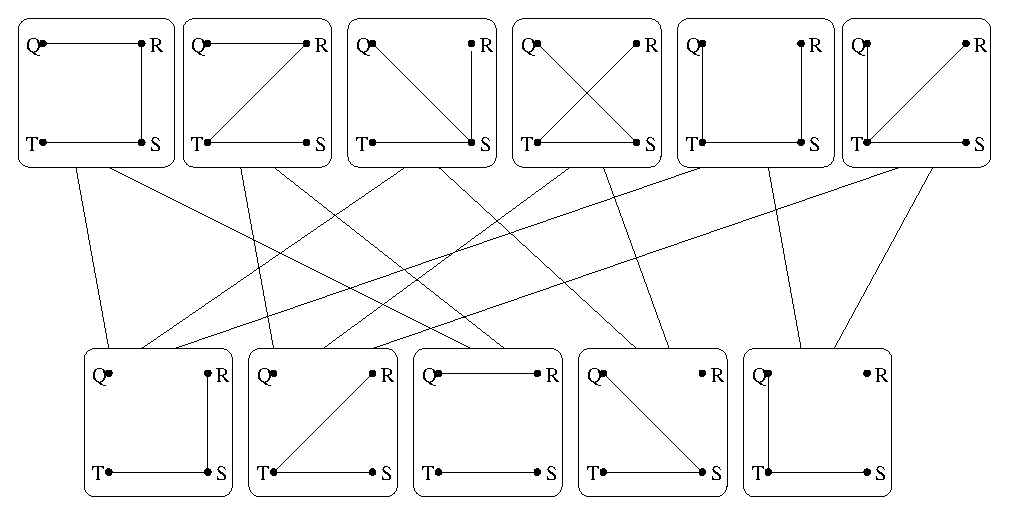
\includegraphics{figures/conn2.eps}
\caption{\label{fi:gc} Illustration of Theorem \ref{th:gc}}
\end{center}
\end{figure}

For the classical case connectivity is known to be evasive
\cite{felsner92complexity}.  If this lower bound is known elsewhere for 
the quantum bounded error setting the author is unaware of it.  It is
not known if this lower bound is asymptotically tight in the bounded
error setting.  It seems reasonable that this bound could be tight,
given the quadratic speedups realized by AND and OR.  Then again it
also seems reasonable that there is no asymptotic speedup as is the
case for MAJORITY and PARITY.

\subsection{Bipartiteness}
\label{sec:bip}

A second fundamental non-trivial monotone graph property is whether a
graph is bipartite.  This graph property is also evasive.

\begin{theorem}
\label{th:nbpt}
$\Omega(V)$ oracle queries are required to decide whether a simple
undirected graph is bipartite.
\end{theorem}

\begin{proof}
We apply Lemma \ref{lm:1xky}, we will only consider simple undirected
graphs with $V \ge 3$.  

Let $x$ be the complete bipartite graph with the first $\left\lfloor
V/2 \right\rfloor$ vertices and second $\left\lceil V/2 \right\rceil$
vertices forming the partitions.  Observe that adding any edge to $x$
results in a non-bipartite graph.  There are
\[
\frac{V(V-1)}{2} - {\left\lfloor\frac{V}{2}\right\rfloor} {\left\lceil\frac{V}{2}\right\rceil} 
= \Theta(V^{2})
\]
such graphs, as there are $V(V-1)/2$ possible edges, $\left\lfloor
V/2\right\rfloor \left\lceil V/2\right\rceil$ of which are in $x$.
Lemma \ref{lm:1xky} implies the lower bound $\Omega(\sqrt{V^{2}}) =
\Omega(V)$.
\end{proof}

If this lower bound is known elsewhere the author is unaware of it.
It is not known if this lower bound is asymptotically tight.  

Having seen two fundamental monotone graph properties with lower
bounds potentially quadratically lower than the classical case it is
tempting to believe these lower bounds are tight and that there is
quadratic speedup in the quantum bounded error model for non-trivial
monotone graph properties.  To see this is not the case we need only
examine the non-trivial monotone graph property analogous to MAJORITY.

\section{No Quantum Extension of the Aanderaa-Karp-Rosenberg Conjecture}
\label{sec:arkbad}

The Aanderaa-Karp-Rosenberg conjecture states that all non-trivial
monotone graph properties are evasive in the classical deterministic
setting.  A natural extension of the Aanderaa-Karp-Rosenberg
Conjecture to quantum computing would conjecture all non-trivial
monotone graph properties have the same query complexity, or at least
the same asymptotic query complexity in the bounded error setting.  To
see that no such extension can hold, observe that the following
non-trivial monotone graph properties can be determined by running the
algorithms for OR, AND, and MAJORITY respectively:

\begin{enumerate}
\item Does the graph have at least 1 edge?
\item Is the graph complete?
\item Does the graph have more than half of all possible edges?
\end{enumerate}

Beals et al.\ provide an $O(V)$ oracle query algorithm for computing
the AND or OR of an $O(V^{2})$ bit oracle string in the bounded error
setting \cite{beals98quantum}, and we have a lower bound of
$\Omega(V)$ oracle queries required to compute them from Section
\ref{sec:AOMP}.  We have a lower bound of $\Omega(V^{2})$ oracle 
queries required to compute the MAJORITY of an $O(V^{2})$ bit oracle
string from Section \ref{sec:AOMP}.  Thus some decision problems for
non-trivial monotone graph properties require $\Theta(V)$ oracle
queries and others $\Theta(V^{2})$ in the bounded error setting, and
there is no extension of the Aanderaa-Karp-Rosenberg conjecture to the
quantum bounded error setting.  This does not come as a complete
surprise, as there are quadratic gaps known between the classically
evasive symmetric functions from Chapter \ref{ch:oracle} in the
quantum bounded error setting.  More disappointing is that there are
graph properties for which the quantum bounded error setting can
provide only constant speedup over the classical case.
